\chapter{Dynamic-ion DMC Study of Solid Hydrogen at Megabar Pressures}
\label{chap:hsolid}
\section{Introduction}

% why is hydrogen under pressure interesting?
The properties and phase transitions of hydrogen under megabar pressures are important in diverse fields of study. For astronomy, models of the interior of giant gas planets such as Jupiter and Saturn depend critically on the nature of the molecular liquid to atomic liquid transition (LLT), namely whether it is first-order or continuous~\cite{Hubbard2016,Wahl2017}. For condensed matter, metallic hydrogen holds promise for a room temperature conventional superconductor~\cite{McMahon2011,McMahon2012}. For computational physics, hydrogen remains an important benchmark for both electronic structure~\cite{Motta2017} and ion dynamics methods. With no need for a pseudopotential, simulations of hydrogen avoid a significant source of bias. However, the low mass of the nuclei necessitates quantum treatment of the lattice degree of freedom, often beyond the harmonic approximation, in accurate simulations.

\begin{figure}[h]
\centering
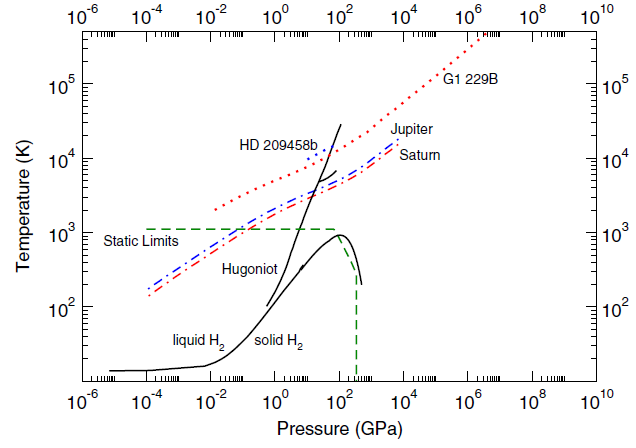
\includegraphics[width=0.6\linewidth]{mcmahon-phases}
\caption{Partial phase diagram of hydrogen on log-log scale~\cite{McMahon2012rmp}.}
\end{figure}

% what controversies are there in experiment?
Established experimental results on high-pressure hydrogen are limited. At room temperature and below, diamond anvil cell (DAC) is the dominant apparatus to achieve such high pressures. Small size of the cell and fragility of the sample limit experimental probes to low-power optics such as infrared and Raman spectroscopy\cite{RangaI.F.2017}. Hydrogen is a weak scatterer of X-Rays~\cite{Zha2014}, thus excluding this excellent tool for structural determination in most experiments. Only recently has X-ray analysis been performed up to 254 GPa~\cite{Akahama2010,Ji2019}.
At high temperatures, shock wave compression is the main method to achieve megabar pressures. Due to the transient nature of theses experiments, acquiring and analyzing shock-wave data is challenging. Most notably, one cannot directly measure temperature, which may cause misinterpretation of raw data~\cite{Celliers2018,Knudson2004,Knudson2017}.
Given the experimental difficulties, predictive simulations are highly desirable as they can inform and verify experiments~\cite{Pierleoni2016b}.

% what controversies are there in calculations?
Simulation of high-pressure hydrogen is also challenging. Without experimental structural information from X-ray, many theoretical calculations have been performed on structures found in density functional theory (DFT) random structure searches~\cite{Pickard2007}. Constrained by computational cost, these searches are limited to classical protons, causing the methods to miss, for example, saddle-point structures that can be stabilized by nuclear quantum effect~\cite{Monserrat2016}.
%Most theoretical studies of high-pressure hydrogen suffer a similar dilemma between accuracy and practicality.
%On the one hand,
Predictive simulations of hydrogen require accurate methods both in the description of the electronic ground-state Born-Oppenheimer (BO) potential energy surface (PES) and in the inclusion of nuclear quantum effect beyond the quasi-harmonic approximation.
%On the other hand, to explore such large pressure and temperature ranges using first-principle methods is not only time consuming, but also prone to other limitations such as inadequate treatment of finite-size effect, nuclear quantum effect, and simulation timescale. Further, some experimentally measurable properties, such as emission, absorption, infrared, and Raman spectra, heat conductivity, and diffusion constants are difficult to calculate in the most accurate electronic methods, e.g., DMC.
The popular Perdew-Burke-Ernzerhof (PBE) density functional in DFT erroneously predicts some molecular structures to be metallic~\cite{Drummond2015}. However, its use in conjunction with Classical molecular dynamics (MD) results in reasonable transition pressure for the LLT at certain temperatures due to error cancellation~\cite{Morales2013a}.
This and other fortuitous cancellations of error has led many to believe that the PBE functional provides a good description of solid hydrogen and caused much confusion in the community. PBE predicts a conductive molecular structure above 200 GPa, a molecular-to-atomic transition around 300 GPa~\cite{McMinis2015}, and low-temperature superconducting liquid. All these predictions contradict experimental evidence. Systematic benchmark of the PES from various DFT functionals against QMC found the vdW-DF1 functional to be the most accurate for molecular hydrogen~\cite{Clay2016}. However, this functional has yet to gain widespread adoption due to its higher computational cost and lower popularity compared to PBE.

In this chapter, I will focus on the solid phases of hydrogen. Sec.~\ref{sec:hsolid-expt} summarizes experimental observations, Sec.~\ref{sec:hsolid-calcs} summarizes relevant computational studies,
Sec.~\ref{sec:hsolid-methods} details the approach taken in this study,
and Sec.~\ref{sec:hsolid-results} presents the computational results.

\subsection{Experiments}
\label{sec:hsolid-expt}

As element number one with the simplest atomic structure, hydrogen has surprisingly complex phases at megabar pressures.
Further complicating matters, the phase diagram depends on the isotopes, e.g., hydrogen H, deuterium D, and spin isomers of molecular hydrogen.
The proton spins anti-align to form a singlet para-hydrogen (p-H$_2$), whereas they align to form a triplet in ortho-hydrogen (o-H$_2$).
To clarify the narrative, I will first introduce the well-established phases in pure samples, then discuss changes due to isotopic and ortho-para conversion.

For pure p-H$_2$ at low temperature (5$\sim$10 K), three solid phases are well-established. The low-pressure phase (LP) below 100 GPa is a molecular crystal having spherically symmetric H$_2$ molecules on hcp lattice sites. Above 110 GPa, hydrogen enters a broken-symmetry phase (BSP), where anisotropic intermolecular interactions favor the $J=2$ $v=1$ vibrational state of the H$_2$ molecules rather than the spherically symmetric $J=0$ $v=1$ state~\cite{Lorenzana1990}. Above 160 GPa, after crossing a first-order transition, one finds an orientationally-ordered phase known as the A phase (H-A)~\cite{Lorenzana1989}.

The transition from LP to BSP phase is sensitive to isotope and nuclear spin. o-D$_2$, HD, and p-H$_2$ enters the BSP at 28 GPa~\cite{Silvera1981}, 70 GPa~\cite{Chijioke2006}, and 110 GPA~\cite{Lorenzana1990}, respectively. o-H$_2$ and p-D$_2$ have a hcp to fcc transition at ambient pressure. In contrast, the transition to the A phase is fairly robust across isotope and spin isomer variants. HD, o-D$_2$, and p-H$_2$ all enter the A phase between 150 and 160 GPa~\cite{Hemley1988,Lorenzana1989,Cui1994,Chijioke2006}. The phase lines for o-D$_2$ and HD are shown in Fig.~\ref{fig:hsolid-phases123}. The p-H$_2$ LP-BSP phase line near 100 GPa is not shown. The size and shape of the BSP is the only difference between the phase diagrams of p-H$_2$, o-D$_2$, and HD.

\begin{figure}[h]
\centering
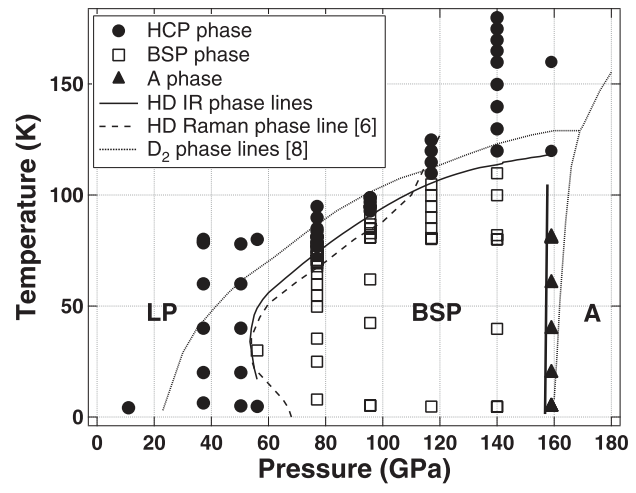
\includegraphics[width=0.6\linewidth]{phases123}
\caption{Phase diagram of o-D$_2$ and HD below 200 K and 200 GPa~\cite{Chijioke2006}.}
\label{fig:hsolid-phases123}
\end{figure}

Transitions to these orientationally ordered phases are detected by changes in Raman and IR spectra. As shown in Fig.~\ref{fig:hsolid-p-h2-bsp}, during the LP to BSP transition, one can observe clear broadening and weakening of the low-frequency roton bands around 350 cm$^{-1}$ and an associated small (15 cm$^{-1}$) discontinuity in the position of the vibron peak, which is about 4150 cm$^{-1}$ near the transition pressure 110 GPa~\cite{Lorenzana1990}. Upon further increase of pressure past 160 GPa, a much larger discontinuity of the Raman vibron (100 cm$^{-1}$) signals the onset of the A phase~\cite{Hemley1988,Lorenzana1989}. A direct transition from H-A back to the LP phase can be achieved by raising temperature. Across this transition, the intensities of the libron bands decrease discontinuously~\cite{Lorenzana1990}.

\begin{figure}[h]
\centering
\begin{minipage}{0.38\columnwidth}
\centering
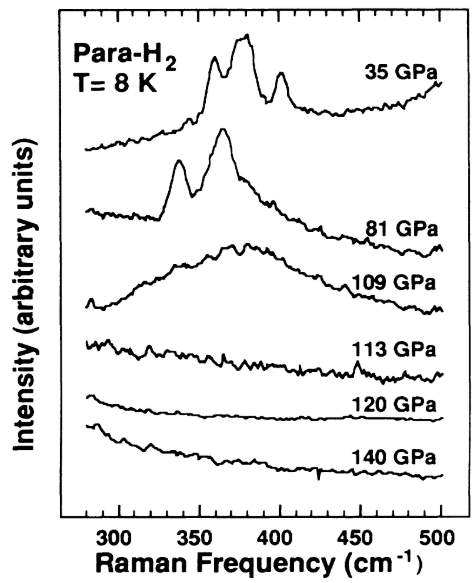
\includegraphics[width=\columnwidth]{p-h2-bsp-rotons}
(a) rotons
\end{minipage}
\begin{minipage}{0.58\columnwidth}
\centering
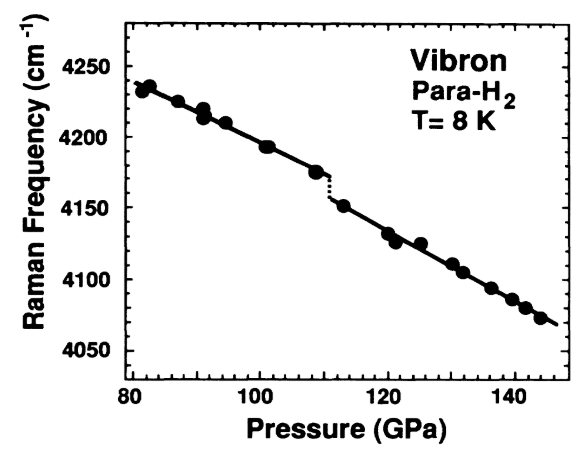
\includegraphics[width=\columnwidth]{p-h2-bsp-vibron}
(b) vibron
\end{minipage}
\caption{Roton and vibron changes in p-H$_2$ across the BSP transition~\cite{Lorenzana1990}.}
\label{fig:hsolid-p-h2-bsp}
\end{figure}

The optical signatures for the LP to BSP transition in o-D$_2$ are qualitatively similar to those in p-H$_2$. The vibron decreases discontinuously by 3 cm$^{-1}$ rather than 15 cm$^{-1}$, while the roton bands broaden and weaken near the transition pressure of 28 GPa rather than 110 GPa~\cite{Silvera1981}. Further confirmation of these two phase transitions were later obtained from IR absorption spectra~\cite{Cui1994}. Three absorption peaks appear around 3150 cm$^{-1}$ upon entering the BSP phase and are replaced by a single broad peak at the same frequency range when the A phase is reached. The same signatures were used to identify the BSP and A phases of HD at 70 and 160 GPa, respectively~\cite{Chijioke2006}.
In the A phase, the rather broad and pressure-independent roton band weakens, disappears, and is replaced by a few sharp and strongly pressure-dependent peaks in the frequency range 100$\sim$700 cm$^{-1}$~\cite{Goncharov1998}.
These new modes are considered to be lattice libration modes due to their pressure dependence.

%As pressure increases, anisotropic intermolecular interactions mix the free roton states until the ground state distorts and molecules become orientationally ordered to lower potential energy. This broken-symmetry phase (BSP) or phase II, stable under 140 K, is considered a quantum phase based on observed strong isotope shift of the transition pressure. o-D$_2$ reaches the BSP phase at as low as 28 GPa at 1.1 K~\cite{Silvera1981}.

Phases with mixed ortho-para concentrations of H$_2$ are labeled I, II, and III~\cite{Dias2016,Dias2019}, which correspond to the LP, BSP, and H-A phases of pure p-H$_2$, respectively.
As shown in Fig.~\ref{fig:hsolid-phases}, at 300 K and above 220 GPa, we enter yet another solid phase IV, characterized by a splitting of the vibron peak~\cite{Zha2013}.
Both theory and experiment suggest that phase IV consists of alternating layers having rather different in-plane structures, possibly two types of molecules.
Below 100 K and above 350 GPa, molecular hydrogen becomes semi-metallic, possibly due to the closure of an indirect band gap~\cite{Eremets2019}.
Then, above 425 GPa, all IR radiation is absorbed indicating a closure of the direct band gap~\cite{Loubeyre2020}.
Finally, at sufficiently high pressures, the hydrogen molecules will dissociate to form an atomic solid, reportedly at 495 GPa~\cite{Silvera2017}, although consensus has yet to be reached.

\begin{figure}[h]
\centering
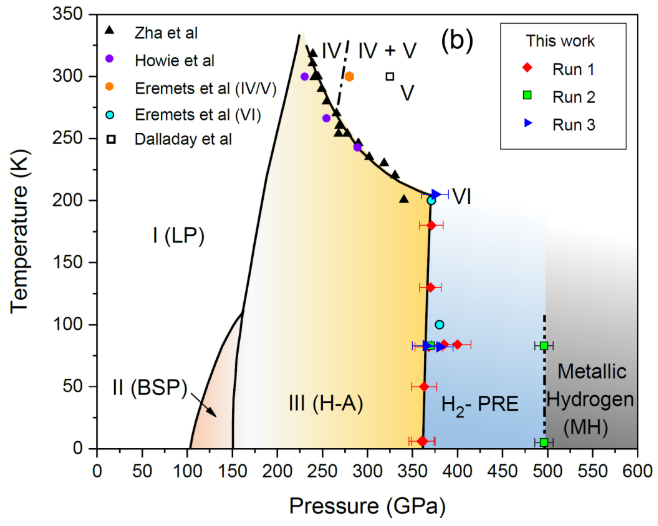
\includegraphics[width=0.6\linewidth]{hsolid-phases}
\caption{Tentative phase diagram of solid hydrogen below 400 K~\cite{Dias2019}.}
\label{fig:hsolid-phases}
\end{figure}

While the phase boundaries of solid hydrogen are reasonably well-established below 400 K and 400 GPa by diamond-anvil cell (DAC) experiments, characterizations of the solid structures are limited. Due to the small scattering cross section and small sample size in DAC experiments, only a handful of X-ray~\cite{Hazen1987,MAO1988,Loubeyre1996,Kawamura2002,Goncharenko2005a,Akahama2010,Ji2019} and only one neutron~\cite{Goncharenko2005a} scattering experiments have been published over the past 40 years. Most of our understanding of solid hydrogen is built upon IR and Raman spectra, which provide partial information on the microscopic details of the solid structures. This lack of definitive structural information poses significant difficulty for both theoretical and experimental understanding of solid hydrogen. Experimentally, this has lead to the misidentification of a triple point as a critical point~\cite{Lorenzana1990,Cui1994}, subtlety in the detection of a new phase~\cite{Eremets2009,Howie2012}, among many debates over interpretation of optical data.

\subsection{Calculations}
\label{sec:hsolid-calcs}

Early computational studies of solid hydrogen rely on assumed crystal structures from known high-pressure phases of other materials or simple symmetry and energetic arguments. Even before the observation of the oriented A phase of solid hydrogen~\cite{Hemley1988}, S. Raynor~\cite{Raynor1987} used Hartree-Fock and perturbation theory to show that the molecular hexagonal closed packed structure with H$_2$ molecules aligned along the c-axis (mhcp-c) is more energetically favorable than previous considered cubic structures.
While a promising candidate for phase III~\cite{Barbee1989}, the mhcp-c structure has an early band overlap, rendering it metallic below 150 GPa, resists compression along the c-axis, and has no IR-active vibron~\cite{Kaxiras1991,Kaxiras1992}, all in contradiction with experimental evidence.
Thus, E. Kaxiras \textit{et al.}~\cite{Kaxiras1991} explored different orientations of H$_2$ molecules in the 2-atom hcp unit cell and found a more energetically favorable insulating structure with molecules oriented $\sim$60$^{\circ}$ from the c-axis.
This static-lattice LDA study was later validated by a dynamic-lattice QMC calculation~\cite{Natoli1995}, and the structure named mhcp-o.
In addition to the hcp structures, H. Nagara and T. Nakamura~\cite{Nagara1992} proposed various rutile structures by minimizing the static-lattice electric quadrupole-quadrupole (EQQ) interactions, while B. Edwards, N. W. Ashcroft, and T. Lenosky~\cite{Edwards1996} proposed an orthorhombic layered structure of Cmca symmetry, which turned out to be metallic at pressures relevant to phase III~\cite{Johnson2000}.
This Cmca crystal structure also appeared spontaneously in path integral simulation~\cite{Cui2002}.
These theoretical calculations drove much debate about the fate of phase III at pressures over 300 GPa. Does it become a metallic molecular solid or does it dissociate into an atomic solid without the band gap closing?

In 2007, the advent of random structure searching produced new candidate crystal structures that have lower enthalpy than previous proposals~\cite{Pickard2007}. The insulating layered structure having C2/c symmetry became the main candidates for phase III.
Three diffusion Monte Carlo studies followed to characterize the candidate structures by Azadi \textit{et al.}~\cite{Azadi2014}, McMinis \textit{et al.}~\cite{McMinis2015}, and Drummond \textit{et al.}~\cite{Drummond2015}.
Azadi \textit{et al.} used PBE-optimized geometries and included anharmonic phonon zero-point energy, leading to a molecular dissociation at 374 GPa, from Cmca-12 to I4$_1$/amd.
In contrast, McMinis \textit{et al.} used vdW-DF-optimized geometries and harmonic phonon zero-point energy to predict a dissociation pressure of 447(3) GPa.
In hind sight, the prediction by McMinis \textit{et al.} is in better agreement with subsequent experiments.

On the low pressure side, a new hexagonal candidate structure for phase III was proposed by Monserrat \textit{et al.}~\cite{Monserrat2016} in 2016, then calculated to be more stable than C2/c below 210 GPa~\cite{Azadi2019}.
Bandgap of the C2/c structure shows closure around 460 GPa, when extrapolated from  was IR measurements up to 420 GPa~\cite{Loubeyre2020}, with the most recent DMC calculation in agreement~\cite{Gorelov2019}. This new calculation is at variance with the previous prediction by Azadi \textit{et al.}~\cite{Azadi2019}, presumably due to different treatments of finite-size effects.
Finally, a recent coupled cluster calculation of the molecular candidate structures show good agreement with DMC results~\cite{Liao2019} at the static lattice level, although lattice zero-point energy has yet to be included.

In this chapter, we examine the most promising candidate structures using dynamic-lattice DMC.
This method treats the electrons and ions on the same footing while harnessing the accuracy of DMC.
Lattice vibrations are included beyond the harmonic approximation and nonadiabatic effects can be captured.
The goal is to provide the most accurate properties of the solid hydrogen phases.
%The goal is to combine and improve upon the best methods in all previous QMC studies and provide the most accurate properties of the solid hydrogen phases.

%\subsection{The melting transition and critical point}
%
%The melting temperature of solid hydrogen is typically determined in one of three ways: 1. visual observation of motion due to sample, contaminant, or laser speckle~\cite{Gregoryanz2003}, 2. discontinuous change in the Raman spectrum, e.g. vibron frequency jump, disappearance of librons~\cite{Gregoryanz2003,Subramanian2011,Zha2017}, 3. plateau temperature during laser heating~\cite{Deemyad2008}, and 4. rapid change in interferences pattern~\cite{Eremets2009}.
%As sample size decreases with pressure, visual detection of melting becomes more difficult. Further, the refractive indexes of hydrogen and diamond approach each other around 140 GPa, defeating detection by interference pattern~\cite{Zha2017}.
%The vibron discontinuity caused by melting reduces from $\sim$ 3 cm$^{-1}$ at 10 GPa to $\sim$ 1 cm$^{-1}$ at 45 GPa~\cite{Gregoryanz2003}, making melting detection more difficult at higher pressures.
%Finally, disappearance of librons alone cannot be taken as proof of melting, because it could be due to loss of sample.
%Due to these difficulties, the precise melting temperatures above 100 GPa are debate. Although, there is broad consensus that the melting line increases from 200 K at ambient pressure to $\sim$ 1000 K at 90 GPa, then decreases with increasing pressure.
%
%Melting of $H_2$ solid around 150 GPa is particularly interesting. Shock wave compression data indicate a molecular liquid to atomic liquid transition $\sim$ 1000 K at 150 GPa. Thus, $H_2$ molecules should dissociate almost immediately after the solid melts. Eremets and Trojan observed a shark drop in measured resistivity as the $H_2$ solid melts at 146 GPa~\cite{Eremets2009}. This observation is consistent with the current liquid-liquid transition (LLT) line.